\documentclass{article}
\usepackage{amsmath,amssymb,amsthm,kotex,paralist,mathrsfs,centernot,marvosym}
\newcounter{num}[section]
\newcommand{\defi}[1]
{\bigskip\noindent\refstepcounter{num}\textbf{정의 \arabic{section}. \arabic{num}) #1}\par}
\newcommand{\theo}[1]
{\bigskip\noindent\refstepcounter{num}\textbf{정리 \arabic{section}. \arabic{num}) #1}\par}
\newcommand{\axio}[1]
{\bigskip\noindent\refstepcounter{num}\textbf{공리 \arabic{section}. \arabic{num}) #1}\par}

\newcommand{\notiff}{%
  \mathrel{{\ooalign{\hidewidth$\not\phantom{"}$\hidewidth\cr$\iff$}}}}
\newcommand{\LHS}{\text{LHS}}
\newcommand{\RHS}{\text{RHS}}
\newcommand{\irange}{\ensuremath{1\le i\le n}}
\newcommand{\jrange}{\ensuremath{1\le j\le n}}
\newcommand{\bb}[2]{\ensuremath{(^{#1}_{#2})}}
\newcommand{\cc}[2]{\ensuremath{_{#1}C_{#2}}}

\renewcommand{\figurename}{그림.}
\renewcommand{\proofname}{증명.}
\renewcommand{\contentsname}{목차}
\renewcommand\emph{\textbf}

%%%
\begin{document}

\title{현빈}
\author{}
\date{2014. 11. 14 木\(\sim\)}
\maketitle
\tableofcontents
\newpage

%%
\setcounter{section}{1}
\section{정수의 나누어떨어짐 특성}

%
\defi{자연수와 정수\label{02_natural_and_integer}}
\begin{align*}
\mathbb N&=\{1,2,3,\cdots\}\\
\mathbb Z&=\{\cdots,-3,-2,-1,0,1,2,3,\cdots\}
\end{align*}
라고 하자.
그러면
\[
\begin{cases}
x\text{는 \emph{자연수}이다.}	&\iff x\in\mathbb N\\
x\text{는 \emph{정수}이다.}		&\iff x\in\mathbb Z
\end{cases}
\]

%
\defi{십진법 숫자의 표기}
10보다 작은 자연수 \(a\), \(b\), \(c\)에 대해 \(\overline{abc}\)를 \(\overline{abc}=100a+10b+c\)로 정의하자.
마찬가지로 10보다 작은 \(k\)개의 자연수 \(a_0\), \(a_1\), \(a_2\), \(\cdots\), \(a_k\)에 대해 \(\overline{a_ka_{k-1}\cdots a_1a_0}\)를
\[
\overline{a_ka_{k-1}\cdots a_1a_0}
=a_k\cdot10^k+a_{k-1}\cdot10^{k-1}+\cdots+a_1\cdot10^1+a_0\cdot10^0
\]
로 정의하자(\(10^0=1\)).

%
\defi{나누어떨어짐(divisibility)}
두 자연수 \(a\), \(b\)에 대해 \(b=ak\)를 만족시키는 자연수 \(k\)가 존재하면 \(b\)는 \(a\)로 \emph{나누어떨어진다}고 말하고, 이를 기호로 \(a\mid b\)라고 한다.

%
\defi{소수(prime, 素數)}
자연수 \(p\neq1\)에 대해 \(a\mid p\)일 때 \(a=p\)이면 \(p\)는 \emph{소수}이다.
즉 \(1\)이 아닌 약수가 자기 자신밖에 없으면 소수이다.

%
\theo{}
소수는 무한히 많이 존재한다.
\begin{proof}
귀류법으로 증명이 가능하다.
36단원에서 증명하겠다.
\end{proof}

%
\theo{산술의 기본정리(The Fundamental Theorem of Arithmetic)\label{02_TFTA}}
임의의 자연수는 소인수분해될 수 있다.
또 소인수분해가 되는 방식은 유일하다.
즉 자연수 \(A\)에 대해
\[A={p_1}^{k_1}\cdot{p_2}^{k_2}\cdot\cdots\cdot{p_n}^{k_n}\]
를 만족시키는 \(p_i\), \(k_i\)들이 유일하게 존재한다.
\begin{proof}
당연해 보이는 정리이고 아주 중요한 정리이지만 증명하기가 쉽지는 않다.
대학 수준의 수학을 이용하면 증명 가능하다.
\end{proof}

%
\theo{\label{02_divsum}}
자연수 \(a\), \(b\), \(c\)에 대해 \(a\mid b\), \(a\mid c\)이면 \(a\mid (b+c)\)이다.
\begin{proof}
\(b=ak\), \(c=al\)을 만족시키는 자연수 \(k\), \(l\)이 존재한다.
그러면 \(b+c=a(k+l)\)이고 이 때 \(k+l\)은 자연수이다.
\end{proof}

%
\theo{\label{02_divdif}}
자연수 \(a\), \(b\), \(c\)(b>c)에 대해 \(a\mid b\), \(a\mid c\)이면 \(a\mid b-c\)이다.
\begin{proof}
\(b=ak\), \(c=al\)을 만족시키는 자연수 \(k\), \(l\)이 존재한다.
그러면 \(b-c=a(k-l)\)이고 이 때 \(k-l\)은 정수이다.
\(k-l=0\)이면 \(b=c\)이 된다.
또 \(k-l<0\)이면 \(b<c\)가 된다.
따라서 \(k-l\)은 자연수이다.
\end{proof}

%
\theo{\label{02_transitivity of divisibility}}
자연수 \(a\), \(b\)에 대해 \(a\mid b\), \(b\mid c\)이면 \(a\mid c\)이다.
\begin{proof}
\(b=ak\), \(c=bl\)을 만족시키는 자연수 \(k\), \(l\)이 존재한다.
그러면 \(c=(ak)l=a(kl)\)이고 \(kl\)은 자연수이므로 \(a\mid c\)이다.
\end{proof}

%
\theo{\label{02_prime division}}
\(p\mid ab\)이고 \(p\nmid a\)이면 \(p\mid b\)이다.
\begin{proof}
정리 \thesection. \ref{02_TFTA}로부터 당연하다.
\end{proof}

%
\theo{\label{02_two-prime division}}
소수 \(p\), \(q(\neq p)\), 자연수 \(a\)에 대해
\[p\mid a\:\&\:q\mid a\iff pq\mid a\]
이다.
\begin{proof}
(\(\Leftarrow\)) 정리 2. \ref{02_transitivity of divisibility}로부터 당연하다.
(\(\Rightarrow\)) 정리 2. \ref{02_TFTA}로부터 당연하다.
\end{proof}

%
\theo{\label{02_divisor_decomposition}}
\(ab\mid c\)이면 \(a\mid c\)이고 \(b\mid c\)이다.
\begin{proof}
c=(ab)k인 자연수 \(k\)가 존재하며 이를 \(c=a(bk)\)꼴로 다시 쓸 수 있다.
따라서 \(a\mid c\)이다.
마찬가지로 \(b\mid c\)이다.
\end{proof}

%
\theo{}
세 자리의 자연수 \(\overline{abc}\)에 대해\\
(1) \(2\mid \overline{abc}\iff2\mid c\)\\
(2) \(5\mid \overline{abc}\iff5\mid c\)\\
(3) \(4\mid \overline{abc}\iff4\mid \overline{bc}\)\\
(4) \(25\mid \overline{abc}\iff25\mid \overline{bc}\)\\
이다.
\begin{proof}
(1) \(2\mid 100a+10b\)이므로 정리 2.\ref{02_divsum}, 정리 2.\ref{02_divdif}에 의해
\[2\mid \overline{abc}\iff2\mid100a+10b+c\iff2\mid c\]
이다.
(2)도 마찬가지로 증명할 수 있다.
(3) \(4\mid100a\)이므로 정리 2.\ref{02_divsum}, 정리 2.\ref{02_divdif}에 의해
\[4\mid\overline{abc}\iff4\mid100a+10b+c\iff2\mid10+c\]
이다.
(4)도 마찬가지로 증명할 수 있다.
\end{proof}

%
\theo{}
일반적으로 \(n+1\)자리의 자연수 \(\overline{a_na_{n-1}\cdots a_1a_0}\)에 대해, 자연수 \(k\)가 \(k\le n\)을 만족시킬 때
\begin{align*}
2^k\Big|\;\overline{a_na_{n-1}\cdots a_1a_0}&\iff2^k\Big|\;\overline{a_{k-1}\cdots a_1a_0}\\
5^k\Big|\;\overline{a_na_{n-1}\cdots a_1a_0}&\iff5^k\Big|\;\overline{a_{k-1}\cdots a_1a_0}
\end{align*}
이다.
\begin{proof}
증명생략.
\end{proof}

%
\theo{\label{02_div_by_3}}
네 자리의 자연수 \(\overline{abcd}\)에 대해\\
(1) \(3\mid\overline{abcd}\iff 3\mid a+b+c+d\)\\
(2) \(9\mid\overline{abcd}\iff 9\mid a+b+c+d\)\\
(3) \(27\mid\overline{abcd}\notiff 27\mid a+b+c+d\)
\begin{proof}
(1) \(3\mid999a+99b+9c\)이므로 정리 2.\ref{02_divsum}, 정리 2.\ref{02_divdif}에 의해
\[3\mid\overline{abcd}\iff3\mid 1000a+100b+10c+d\iff3\mid a+b+c+d\]
이다.
마찬가지의 방법으로 (2)도 성립한다.
(3) \(\overline{abcd}=9945\)이면 \(27\nmid9945\)이고 \(27\mid9+9+4+5\)이다.
\end{proof}

일반적으로 자연수 \(n\)에 대해서 \(n\)자리의 자연수에 대해서도 정리 \thesection. \ref{02_div_by_3}에 해당하는 정리가 성립한다(cf. p33, ④).



%%
\newpage
\section{절댓값에 관한 문제}

%
\theo{절댓값기호\label{03_absolute value}}
실수 \(a\)에 대해
\[
|a|=
\begin{cases}
a&(a\ge0)\\
-a&(a<0).
\end{cases}\]

%
\theo{\label{03_minus absolute value}}
실수 \(a\)에 대해 \(|-a|=|a|\)이다.
\begin{proof}
\(a>0(\therefore -a<0)\)이면 \(|-a|=-(-a)=a=|a|\).
\(a=0\)이면 \(|-a|=|-0|=|0|=|a|\).
\(a<0(\therefore -a>0)\)이면  \(|-a|=-a=|a|\).
\end{proof}

%
\theo{\label{03_iff condition absolute value}}
실수 \(a\)에 대해\\
(1) \(|a|=a\iff a\ge0\),\\
(2) \(|a|=-a\iff a\le0\).
\begin{proof}
(\(\Rightarrow\))
\(|a|=a\)라고 가정하자.
\(a<0\)이면 \(-a=a\)이고, 따라서 \(a=0\), 모순.
따라서 \(|a|=a\)이면서 \(a<0\)일 수 없다.
즉 \(a\ge0\)이어야 한다.
(\(\Leftarrow\))
정의 \thesection. \ref{03_absolute value}로부터 당연하다.

(2) 정리 \thesection. \ref{03_minus absolute value}, 정리 \thesection. \ref{03_iff condition absolute value} (1)에 의해
\begin{align*}
|a|=-a
&\;\;\stackrel{정리 \thesection. \ref{03_minus absolute value}}{\iff}
|-a|=-a\\
&\stackrel{정리 \thesection. \ref{03_iff condition absolute value} (1)}{\iff}
-a\ge0\\
&\;\;\iff
a\le 0
\end{align*}
\end{proof}

%
\theo{}
실수 \(a\), \(a_i(1\le i\le n)\)에 대해\\
(1) \(|a|\ge 0\).\\
(2) \(|a|=0\iff a=0\).\\
(3) \(|a_1|+\cdots+|a_n|=0\iff a_1=0\;\&\;\cdots\;\&\;a_n=0\).
\begin{proof}
정의 \thesection. \ref{03_absolute value}로부터 당연하다.
\end{proof}

%
\theo{절댓값의 곱\label{multiplication of absolute value}}
실수 \(a\), \(b\)에 대해 \(|a|\cdot|b|=|ab|\)가 성립한다.
\begin{proof}
\begin{enumerate}[i)]
\item
\(a\) 혹은 \(b\)가 0인 경우 ; \(\LHS=\RHS\)
\item
\(a>0\:\&\:b>0\) ; \(\LHS=ab=\RHS\)
\item
\(a>0\:\&\:b<0\) ; \(\LHS=a(-b)=-ab=\RHS\)
\item
\(a<0\:\&\:b>0\) ; \(\LHS=(-a)b=-ab=\RHS\)
\item
\(a<0\:\&\:b<0\) ; \(\LHS=(-a)(-b)=\RHS\)
\end{enumerate}
\end{proof}

%
\theo{절댓값의 합, 삼각부등식(Triangular inequality)\label{03_triangular ineq}}
실수 \(a\), \(b\)에 대해
\begin{enumerate}[(1)]
\item
\(|a+b|\le|a|+|b|\)
\item
\(|a+b|=|a|+|b|\iff ab\ge0\).
\end{enumerate}
\begin{proof}
(1) 
i) \(a\) 혹은 \(b\)가 0인 경우 ; 일반성을 잃지 않고 \(b=0\)이라고 하자.
그러면 \(\LHS=|a+0|=|a|=|a|+0=\RHS\).
ii) \(a>0\), \(b>0\)인 경우 ; \(\LHS=a+b=\RHS\).
iii) \(a<0\), \(b<0\)인 경우 ; \(\LHS=-(a+b)=(-a)+(-b)=\RHS\).
iv) \(a\), \(b\) 중 하나는 양수, 하나는 음수인 경우 ; 일반성을 잃지 않고 \(a>0\), \(b<0\)이라고 하자.
\(|a|=|b|\)이면, \(\LHS=|0|=0<a-b=\RHS\).
이제 \(|a|\neq|b|\)인 경우를 고려하자.
일반성을 잃지 않고 \(|a|>|b|\)라고 가정할 수 있다.
즉 \(a+b>0\).
따라서 \(\LHS=a+b<a-b=\RHS\).

(2) (1)의 증명과정으로부터 당연하다.
\end{proof}

%
\theo{수직선 상에서의 거리\label{03_distance}}
수직선 상의 두 점 \(A\), \(B\)의 좌표가 각각 \(a\), \(b\)일 때, \(A\)와 \(B\) 사이의 거리인 \(d(A,B)\)는 다음과 같이 정의한다.
\[d(A,B)=|a-b|.\]

%
\theo{\label{03_distance property}}
수직선 위의 세 점 \(A\), \(B\), \(C\)에 대해 다음이 성립한다.
\begin{enumerate}[(1)]
\item
\(d(A,B)=d(B,A)\)
\item
\(d(A,B)+d(B,C)\le d(A,C)\).
\end{enumerate}
즉, 실수 \(a\), \(b\), \(c\)에 대해
\begin{enumerate}[(1)]
\item
\(|a-b|=|b-a|\)
\item
\(|a-b|+|b-c|\le |a-c|\)
\end{enumerate}
가 성립한다.

\begin{proof}
각각 정리 3. \ref{03_minus absolute value}와 정리 3. \ref{03_triangular ineq}로부터 당연하다.
\end{proof}

%
\theo{부분분수(Partial Fraction)\label{03_partial_fraction}}
실수 \(a\), \(b\), 정수 \(n\)에 대해(\(a\neq b\), \(n\neq1\), \(n\neq0\))
\begin{enumerate}[(1)]
\item
\(\frac1{n(n+1)}=\frac1n-\frac1{n+1}\)
\item
\(\frac1{ab}=\frac1{b-a}\left(\frac1a-\frac1b\right)\)
\end{enumerate}
가 성립한다.



%%
\newpage
\section{미지수가 1개인 일차방정식과 부등식}

%
\defi{일차방정식과 일차부등식}
실수 \(a\neq0\), \(b\)에 대해 \(ax+b=0\) 꼴의 등식을 \emph{일차방정식}이라고 한다.
또 \(ax+b>0\), \(ax+b<0\), \(ax+b\le0\), \(ax+b\ge0\) 꼴의 부등식을 \emph{일차부등식}이라고 한다.

%
\theo{\(ax+b=0\)꼴의 등식의 풀이\label{04_linear eq. solution}}
\(a\), \(b\)가 실수일때,
\begin{enumerate}[i)]
\item
\(a\neq0\)이면 \(ax+b=0\iff x=-\frac ba\)이다.
\item
\(a=0\), \(b\neq0\)이면 근이 존재하지 않는다(불능不能).
즉, 어떤 실수 \(x\)도 위 등식을 만족시키지 않는다.
\item
\(a=0\), \(b=0\)이면 근이 무수히 많다(부정不定).
즉, 모든 실수 \(x\)에 대해서 위 등식을 만족시킨다.
\end{enumerate}

%
\axio{\label{04_inequality_axiom_1}}
실수는 `\(<\)'로 표기하는 이항관계를 가지며 이를 부등호라고 한다.
\begin{enumerate}[(1)]
\item
실수 \(a\), \(b\)에 대해 \(a<b\)이거나 \(a=b\)이거나 \(a<b\)이다.
\item
실수 \(a\), \(b\), \(c\)에 대해 \(a<b\), \(b<c\)이면 \(a<c\)이다.
\end{enumerate}

%
\axio{\label{04_inequality_axiom_2}}
실수 \(a\), \(b\), \(c\)에 대해
\begin{enumerate}[(1)]
\item
\(a+c<b+c\)이다.
\item
\(c>0\)이면 \(ac<bc\)이다.
\item
\(c<0\)이면 \(ac>bc\)이다.
\end{enumerate}
공리란, 증명할 필요가 없는 문장으로서, 다른 명제(정리)를 증명하는 데 있어 기초가 되는 원리이다.
위에 두 공리에 적힌 내용들을 증명하는 것은 불가능하다.
하지만 실수를 구성할 때에 위의 공리들을 가지고 실수를 정의하기 때문에 참인 명제라고 볼 수 있다.



%%
\newpage
\section{미지수가 2개인 일차연립방정식 및 응용}
%
\defi{다항식\label{05_polynomial}}
(1) 음이 아닌 정수 \(n\)과 실수 \(a_i\) (\irange), (\(a_n\neq0\))에 대해서
\[
a_nx^n+a_{n-1}x^{n-1}+a_{n-2}x^{n-2}+\cdots+a_2x^2+a_1x+a_0
\]
꼴의 식을 `\(x\)에 대한 다항식'이라고 한다.

(2) 음이 아닌 정수 \(m\), \(n\)과 실수 \(a_{ij}\) (\(1\le i\le m\), \jrange, \(a_{mn}\neq0\))에 대해서
\begin{gather*}
a_{mn}x^my^n+a_{m,n-1}x^my^{n-1}+\cdots+a_{m1}x^my+a_{m0}x^m\\
+a_{m-1,n}x^{m-1}y^n+a_{m-1,n-1}x^{m-1}y^{n-1}+\cdots+a_{m-1,1}x^{m-1}y+a_{m-1,0}x^{m-1}\\
\vdots\\
a_{0n}y^n+a_{0,n-1}y^{n-1}+\cdots+a_{01}y+a_{m0}
\end{gather*}
꼴의 식을 `\(x\)와 \(y\)에 대한 다항식'이라고 한다.
예를 들어 \(x^2+x+2\)는 \(x\)에 대한 다항식이고 \(2x^3y^2+x^3y^2-3x^2y^2+x^2+2y-1\)은 \(x\), \(y\)에 대한 다항식이다.

(3) (1)과 (2)의 정의에서, \(a_ix^i\) 혹은 \(a_{ij}x^iy^j\) 각각을 \emph{항}이라고 한다.
또 \(a_i\) 혹은 \(a_{ij}\) 들을 \emph{계수}라고 한다.
그리고 (1)에서 \(n\)을 \emph{차수}라고 하고, (2)에서 \(m\)을 `\(x\)에 대한 차수', \(n\)을 `\(y\)에 대한 차수'라고 한다.
\(a_nx^n\) 혹은 \(a_{mn}x^my^n\)을 \emph{최고차항}이라고 하고, \(a_0\), \(a_{00}\)를 \emph{상수항}이라고 한다.
또 항이 한 개인 다항식을 \emph{단항식}이라고 부른다.

(4) 마찬가지로 세 개 이상의 미지수에 대해서도 다항식을 정의할 수 있다.

%
\defi{연립방정식}
\(n\)개의 미지수의 다항식으로 만들어지는 두 개 이상의 방정식에 대해 최고차수가 \(m\)이면 이 일련의 식들을 일컬어 `\(n\)원 \(m\)차 연립방정식'이라고 한다.
예를 들어
\[
\begin{cases}
x^2+2xy-3y^2=0\\
x+y=7
\end{cases}
\]
은 \(x\), \(y\)에 대한 이원이차연립방정식이고
\[
\begin{cases}
x+y+z=7\\
x+2y+z=8\\
2x+y+z=9
\end{cases}
\]
는 \(x\), \(y\), \(z\)에 대한 삼원일차연립방정식이다.

%
\theo{이원일차연립방정식}
\(a_1\neq0\), \(a_2\neq0\), \(b_1\neq0\), \(b_i\neq0\)인 이원일차연립방정식
\begin{gather}
a_1x+b_1y=c_1\\
a_2x+b_2y=c_2
\end{gather}
은 다음과 같이 풀어낼 수 있다.

i) \(a_1b_2-a_2b_1\neq0\) (i.e. \(\frac{a_1}{a_2}\neq\frac{b_1}{b_2}\))\par
\(b_2\times(1)-b_1\times(2)\)를 계산하면 \((a_1b_2-a_2b_1)x=b_2c_1-b_1c_2\)이다.
이때 \(a_1b_2-a_2b_1\neq0\)이므로
\[x=\frac{b_2c_1-b_1c_2}{a_1b_2-a_2b_1}\]
이다.
마찬가지로 
\(a_1\times(2)-a_2\times(1)\)를 계산하면 \((a_1b_2-a_2b_1)x=a_1c_2-a_2c_1\)이다.
이때 \(a_1b_2-a_2b_1\neq0\)이므로
\[x=\frac{a_1c_2-a_2c_1}{a_1b_2-a_2b_1}\]
이다.

ii) \(a_1b_2-a_2b_1=0\) (i.e. \(\frac{a_1}{a_2}=\frac{b_1}{b_2}\))\par
\(b_2\times(1)-b_1\times(2)\)를 계산하면
\[0\cdot x=b_2c_1-b_1c_2\tag{3}\]
이다.

ㄱ) \(b_2c_1-b_1c_2=0\) (i.e. \(\frac{b_1}{b_2}=\frac{c_1}{c_2}\))이면, 임의의 실수 \(x\)에 대해서 \(y\)를 (1)을 만족시키는 실수인 \(y=\frac{c_1-a_1x}{b_1}\)라고 하면 이러한 \(x\), \(y\)는 (2)도 만족시킨다 ;
\begin{align*}
a_2x+b_2\frac{c_1-a_1x}{b_1}
&=a_2x+\frac{b_2}{b_1}c_1-\frac{b_2}{b_1}a_1x\\
&=a_2x+\frac{c_2}{c_1}c_1-\frac{a_2}{a_1}a_1x\\
&=c_2.
\end{align*}
따라서 연립방정식의 해는 무한히 많다
(부정不定).

ㄴ) \(b_2c_1-b_1c_2\neq0\) (i.e. \(\frac{b_1}{b_2}\neq\frac{c_1}{c_2}\))이면 (3)의 해가 없으므로 연립방정식의 해도 존재하지 않는다(불능不能).

%
\theo{이원연립방정식의 기하학적 해석\label{05_geometric_interpretation}}
\(f(x,y)\), \(g(x,y)\)가 \(x\), \(y\)에 대한 다항식일 때, 연립방정식
\[
\begin{cases}
f(x,y)=0\\
g(x,y)=0
\end{cases}
\]
의 해의 집합을 \(R=\{(x,y)\mid f(x,y)=0,\:g(x,y)=0\}\)은, \(xy\)평면 상의 두 그래프 \(f(x,y)=0\), \(g(x,y)=0\)의 교집합과 같다.

\begin{proof}
\(F=\{(x,y)\mid f(x,y)=0\}\), \(G=\{(x,y)\mid g(x,y)=0\}\)라고 하면, \(F\cap G=R\)이다.
\end{proof}

즉 연립방정식이라는 `대수적인' 문제를 두 도형의 교점을 찾는 `기하학적' 문제로 바꿀 수 있다.
예를 들어, 다음과 같은 이원이차연립방정식이 제시되어 있을 때
\[
\begin{cases}
y=x^2\\
y=x+2
\end{cases}
\]
(즉 \(f(x,y)=y-x^2\), \(g(x,y)=y-x-2\)이다.)
이 방정식의 해의 집합인 \{(-1,2),(2,4)\}은 두 그래프 \(F=\{(x,y)\mid y=x^2\}\)와 \(G=\{(x,y)\mid y=x+2\}\)의 교집합과 같다.
(그림. 1)
\begin{figure}[h]
\center
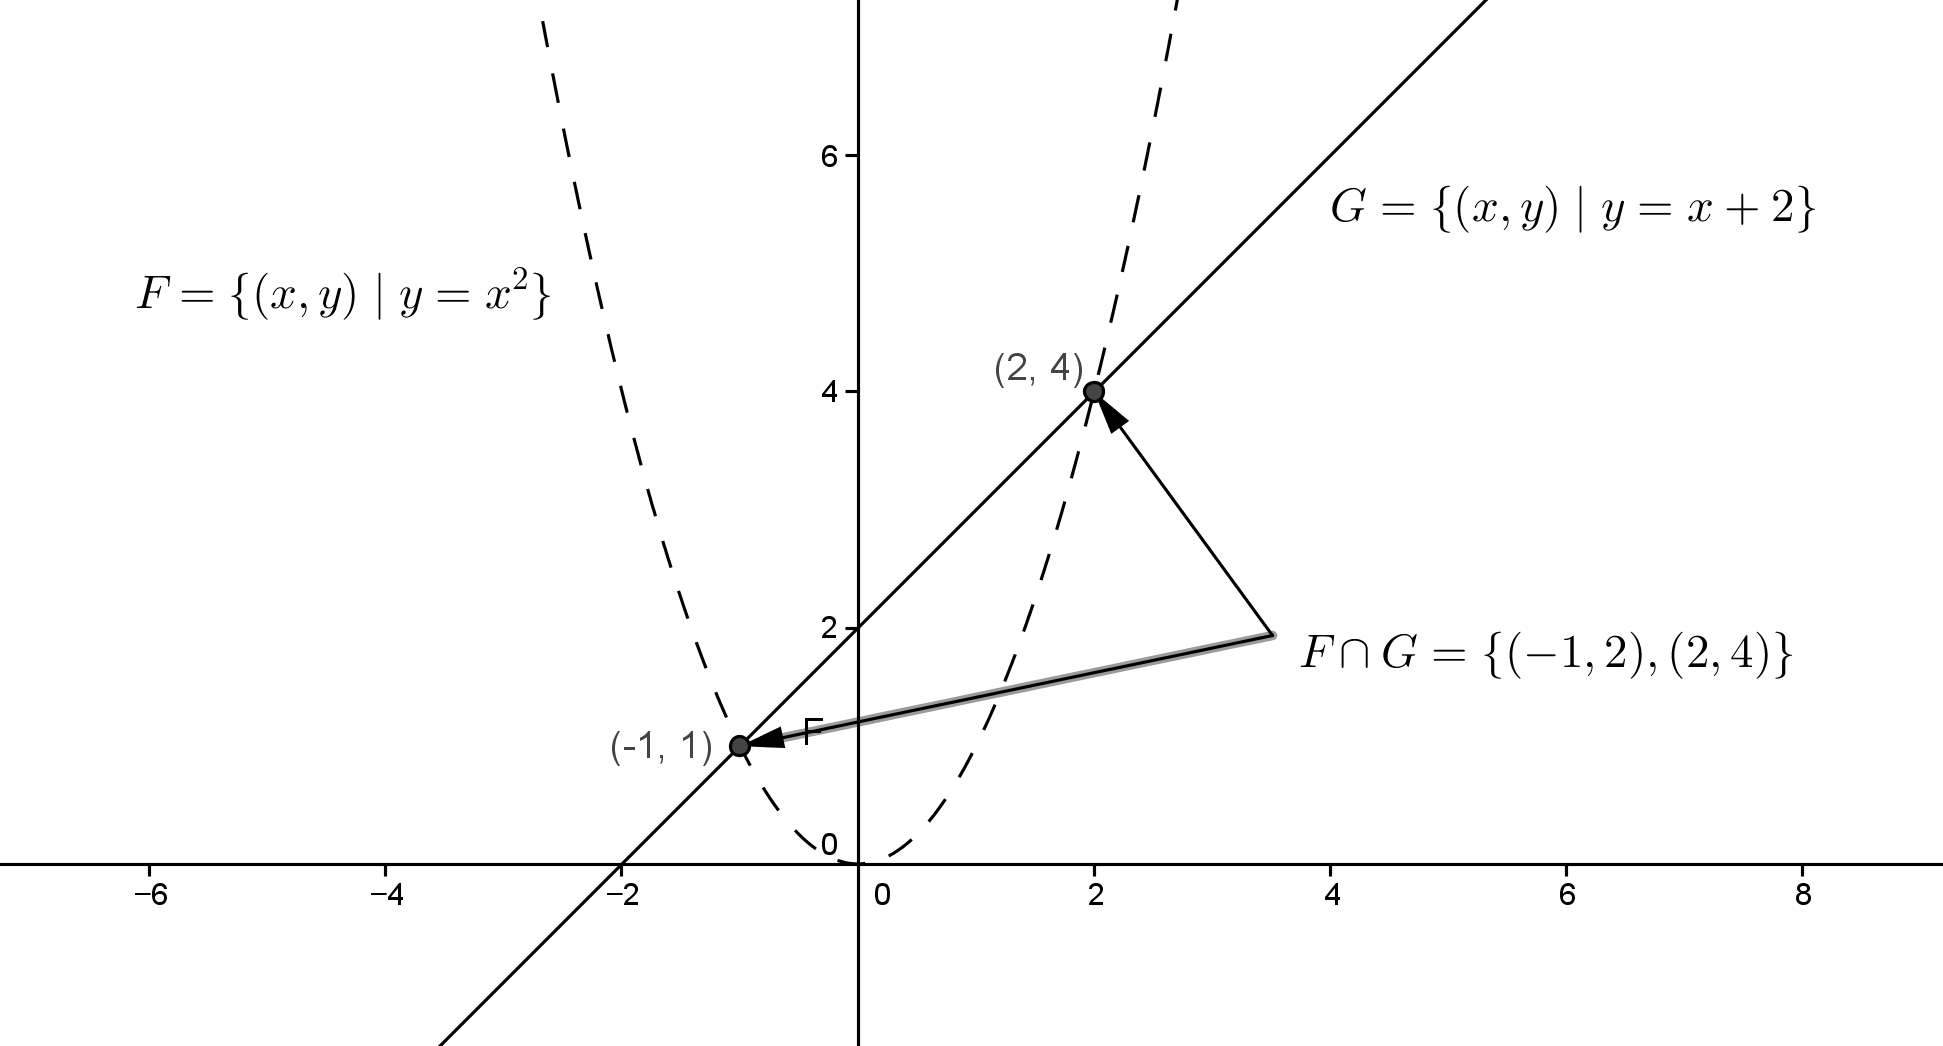
\includegraphics[width=0.7\textwidth]{05_intersects}
\caption{연립방정식 \(y=x+1\), \(y=x^2\)의 기하학적 해석}
\end{figure}



%%
\newpage
\section{정식의 계산}
%
\axio{\label{06_number_axiom}}
실수 \(a\), \(b\)에 대해
\begin{enumerate}[(1)]
\item
\(a+b=b+a\)
\item
\((a+b)+c=a+(b+c)\)
\item
\(ab=ba\)
\item
\((ab)c=a(bc)\)
\item
\(a(b+c)=ab+ac\)
\end{enumerate}
가 성립한다.
공리 4. \ref{04_inequality_axiom_1}, 4. \ref{04_inequality_axiom_2}와 마찬가지로 실수를 정의할 때 사용되는 가정이므로 증명될 수는 없다.
따라서 공리로 치부하겠다.

%
\theo{\label{06_polynomial_theorem}}
다항식 \(A\), \(B\), \(C\)에 대해 
\begin{enumerate}[(1)]
\item
\(A+B=B+A\)
\item
\((A+B)+C=A+(B+C)\)
\item
\(AB=BA\)
\item
\((AB)C=A(BC)\)
\item
\(A(B+C)=AB+AC\)
\end{enumerate}
가 성립한다.

\begin{proof}
다항식(\ref{05_polynomial})에서 미지수에는 실수가 대입되므로 다항식 자체도 하나의 실수라고 생각할 수 있다.
따라서 공리 5. \ref{06_number_axiom}에 의해 성립한다.
\end{proof}

%
\theo{\label{06_square formula}}
실수 \(a\), \(b\), \(c\), \(d\)에 대해서
\begin{enumerate}[(1)]
\item
\((a+b)^2=a^2+2ab+b^2\)
\item
\((a+b+c)^2=a^2+b^2+c^2+2(ab+bc+ca)\)
\item
\((a+b+c+d)^2=a^2+b^2+c^2+d^2+2(ab+ac+ad+bc+bd+cd)\)
\item
\((a_1+\cdots+a_n)^2=
{a_1}^2+\cdots+{a_n}^2+2(a_1a_2+a_1a_3+\cdots a_1a_n+a_2a_3+a_2a_4+\cdots a_2a_n+\cdots+a_{n-1}a_n)\)
\end{enumerate}

%
\defi{\label{06_pascal's_triangle}파스칼Pascal의 삼각형(혹은 양휘揚輝의 삼각형)}
다음과 같이, 0이 아닌 정수 \(n\)에 대해, \(n\)행에 \((n+1)\)개의 숫자를 적되 첫 숫자와 마지막 숫자를 \(1\)로, \(k(1<k<n+1)\)번째 숫자를 \(n-1\)행의 \((k-1)\)번째 숫자와 \(k\)번째 숫자의 합으로 정할 때, 이 숫자들의 삼각형을 \emph{파스칼Pascal의 삼각형} 혹은 \emph{양휘揚輝의 삼각형}이라고 부른다.

이때 \(n\)행의 \(k\)번째 숫자를 %\(_nC_k\)혹은
\((^n_k)\)로 표기한다(\(0\le k\le n\)).
따라서
\begin{gather*}
%_nC_0=_nC_n=1,\qquad_{n-1}C_{k-1}+_{n-1}C_{k}=_nC_k\\
(^n_n)=(^n_0)=1,\qquad(^{n-1}_{k-1})+(^{n-1}_{k})=(^n_k)
\end{gather*}
이다(그림. 2).

\begin{figure}[h]
\center
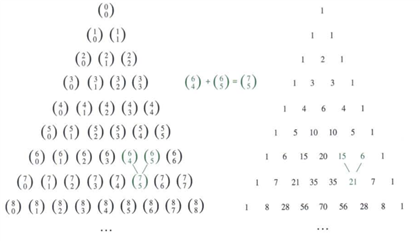
\includegraphics[width=\textwidth]{06_pascal}
\caption{파스칼의 삼각형}
\end{figure}

%
\defi{조합\label{06_combination}}
\cc nk를
\(k=0\) 이거나 \(k=n\)인 경우 \(1\)로 정의하고
\(k\neq0,n\)인 경우 `\(1\), \(2\), \(\cdots\), \(n\)의 \(n\)개의 숫자 중 \(k\)개를 순서에 상관없이 뽑는 경우의 수'로 정의하자.
예를 들어, \(1\), \(2\), \(3\), \(4\)의 \(4\)개의 숫자 중 \(2\)개를 순서에 상관없이 뽑는 경우의 수는 \((1,2),(1,3),(1,4),(2,3),(2,4),(3,4)\)의 \(6\)가지이므로, \(\cc42=6\)이다.

%
\theo{}
\cc nk=\bb nk이다.


\begin{proof}
\(1\), \(2\), \(3\), \(\cdots\), \(n\)의 \(n\)개의 자연수 중 \(k\)개의 자연수를 순서에 상관없이 뽑는 경우의 수는, \(n-1\)개의 자연수 중 \(k\)개의 자연수를 순서에 상관없이 뽑는 경우의 수에 \(n-1\)개의 자연수 중 \(k-1\)개의 자연수를 순서에 상관없이 뽑은 후 \(n\)을 추가하는 경우의 수를 더한 값과 같다.
즉
\[_{n-1}C_{k-1}+_{n-1}C_{k}=_nC_k\]
이다.
또한 \(_nC_0=_nC_n=1\)이므로 \bb nk와 \cc nk의 정의는 완전히 같다.
따라서 \(\bb nk=\cc nk\)이다.
\end{proof}

%
\theo{이항정리(Binomial Theorem)\label{06_binomial_theorem}}
실수 \(a\), \(b\)와 음이 아닌 정수 \(n\)에 대해
\begin{align*}
(a+b)^0&=&\bb00a^0b^0\\
(a+b)^1&=&\bb10a^1b^0+\bb11a^0b^1\\
(a+b)^2&=&\bb20a^2b^0+\bb21a^1b^1+\bb22a^0b^2\\
(a+b)^3&=&\bb30a^3b^0+\bb31a^2b^1+\bb32a^1b^2+\bb33a^0b^3\\
\vdots\\
(a+b)^n&=&\bb{n}0a^nb^0+\bb{n}1a^{n-1}b^1+\bb{n}2a^{n-2}b^2+\cdots+\bb{n}0a^0b^n\\
\end{align*}

\begin{proof}
\((a+b)^n\)의 전개식의 각 항의 \(a\), \(b\)에 대한 차수는 \(n\)이다.
즉 \((a+b)^n\)의 전개식의 각 항은 \(a^kb^{n-k}\)로 표현될 수 있다.
또 항 \(a^kb^{n-k}\)이 나타나는 횟수는, 총 \(n\)번 중 \(k\)번이 순서에 상관없이 선택되는 경우의 수인 \cc nk이다.
\end{proof}

%
\defi{이항전개와 이항계수}
정리 6. \ref{06_binomial_theorem}에서와 마찬가지로 항이 두 개인 식의 거듭제곱을 전개하는 것을 \emph{이항전개}라고 하고, 이때 나타나는 계수들인 \bb nk를 \emph{이항계수}라고 한다.

%
\defi{\label{06_number_division}}
두 자연수 \(A\), \(B\)에 대해서 \(A=BQ+R(0\le R<B)\)인 자연수 \(Q\), \(R\)이 존재할 때 \(Q\)를 \emph{몫(Quotient)}, \(R\)을 \emph{나머지(Remainder)}라고 부른다.
\(A\), \(B\)는 각각 \emph{피제수}, \emph{제수}라고 불린다.

%
\theo{}
정리 6. \ref{06_number_division}의 \(Q\)와 \(R\)은 반드시 존재하며 또 유일하게 존재한다.
\begin{proof}
증명생략.
\end{proof}

%
\defi{\label{06_polynomial_division}}
두 다항식 \(f(x)\), \(g(x)\)에 대해서 \(f(x)=g(x)Q(x)+R(x)\)(\(R(x)\)의 차수\(<g(x)\)의 차수)인 다항식 \(Q(x)\), \(R(x)\)이 존재할 때 \(Q(x)\)를 \emph{몫(Quotient)}, \(R(x)\)을 \emph{나머지(Remainder)}라고 부른다.
\(f(x)\), \(g(x)\)는 각각 \emph{피제수}, \emph{제수}라고 불린다.

%
\theo{}
정리 6. \ref{06_polynomial_division}의 \(Q(x)\)와 \(R(x)\)은 반드시 존재하며 또 유일하게 존재한다.
\begin{proof}
증명생략.
\end{proof}

%
\theo{나머지 정리\label{06_remainder_theorem}}
\begin{enumerate}[(1)]
\item
\(f(x)\)를 \(x-\alpha\)로 나눈 나머지는 \(f(\alpha)\)이다.
\item
\(f(x)\)를 \(ax+b(a\neq0)\)로 나눈 나머지는 \(f(-\frac ba)\)이다.
\end{enumerate}
\begin{proof}
(1) \(f(x)\)를 \(x-\alpha\)로 나누었을 때의 몫을 \(Q(x)\), \(R(x)\)라고 하자.
그러면 \(f(x)=(x-\alpha)Q(x)+R(x)\)로 쓸 수 있다.
이때 \(R(x)\)의 차수는 1차보다 작아야 하므로 상수이다.
따라서 \(R(x)=R\)로 쓰자.
그러면
\[f(x)=(x-\alpha)Q(x)+R\]
이다.
양변에 \(x=\alpha\)를 대입하면 위의 결과를 얻는다.
(2) 또한 같은 방법으로 증명할 수 있다.
\end{proof}

%
\theo{인수정리\label{06_factor_theorem}}
\[(x-\alpha)\mid f(x)\iff f(\alpha)=0.\]
\begin{proof}
정리 6. \ref{06_remainder_theorem}의 증명에서와 마찬가지로 \(f(x)=(x-\alpha)Q(x)+R\)이라고 하면
\[(x-\alpha)\mid f(x)\iff R=0\iff f(\alpha)=0.\]
\end{proof}



%%
\newpage
\section{인수분해(1)}

%
\defi{인수분해}
다항식 \(f(x)\)에 대해서 \(f(x)\)를 두 개 이상의 다항식의 곱 (e.g. \(f(x)=g(x)h(x)\) 혹은 \(f(x)=g(x)h(x)k(x)\), \(\cdots\))으로 변형시키는 과정을 \emph{인수분해}라고 한다.
반대로 주어진 두 개 이상의 다항식의 곱을 합의 형태로 풀어내는 것을 \emph{전개}라고 한다.

%
\theo{인수분해 공식}
실수 \(a\), \(b\), \(c\), \(d\), \(x\)에 대해 다음 식들이 성립한다.
\begin{enumerate}[(1)]
\item
\((a+b)^2=a^2+2ab+b^2\)
\item
\((a-b)^2=a^2-2ab+b^2\)
\item
\(a^2+b^2=(a+b)^2-2ab=(a-b)^2+2ab\)
\item
\((a+b)^2=(a-b)^2+4ab\)
\item
\((x+\frac1x)^2=x^2+\frac1{x^2}+2\)
\item
\((x-\frac1x)^2=x^2+\frac1{x^2}-2\)
\item
\(x^2+\frac1{x^2}=(x+\frac1x)^2-2=(x-\frac1x)^2+2\)
\item
\((x+\frac1x)^2=(x-\frac1x)^2+4\)
\item
\((a-b)(a+b)=a^2-b^2\)
\item
\((x+\frac1x)(x-\frac1x)=x^2-\frac1{x^2}\)
\item
\((x+a)(x+b)=x^2+(a+b)x+ab\)
\item
\((ax+b)(cx+d)=acx^2+(ad+bc)x+bd\)
\item
\((x+a)(x+b)(x+c)=x^3+(a+b+c)x^2+(ab+bc+ca)x+abc\)
\item
\((x-a)(x-b)(x-c)=x^3-(a+b+c)x^2+(ab+bc+ca)x-abc\)
\item
\((a+b+c)^2=a^2+b^2+c^2+2(ab+bc+ca)\)
\item
\(a^2+b^2+c^2=(a+b+c)^2-2(ab+bc+ca)\)
\item
\((a+b)^3=a^3+3a^2b+3ab^2+b^3=a^3+b^3+3ab(a+b)\)
\item
\((a-b)^3=a^3-3a^2b+3ab^2-b^3=a^3-b^3-3ab(a-b)\)
\item
\(a^3+b^3=(a+b)^3-3ab(a+b)\)
\item
\(a^3-b^3=(a-b)^3+3ab(a-b)\)
\item
\(a^3+b^3=(a+b)(a^2-ab+b^2)\)
\item
\(a^3-b^3=(a-b)(a^2+ab+b^2)\)
\item
\((a+b+c)(a^2+b^2+c^2-ab-bc-ca)=a^3+b^3+c^3-3abc\)\\
\(*\;a+b+c=0\)이면 \(a^3+b^3+c^3=3abc\)\\
\(*\;a^2+b^2+c^2-ab-bc-ca=\frac12[(a-b)^2+(b-c)^2+(c-a)^2]\)
\item
\(a^4+a^2b^2+b^4=(a^2+ab+b^2)(a^2-ab+b^2)\).
\end{enumerate}

\begin{proof}
분배법칙을 사용하여 전개해보면 모든 식이 성립한다는 것을 확인할 수 있다.
\end{proof}

%
\theo{cf. 예제 04(p. 68)}
실수 \(a\), \(b\), \(x_i\)(\irange), 자연수 \(n, k\)에 대해
\begin{enumerate}[(1)]
\item
\(a^n-b^n=(a-b)(a^{n-1}+a^{n-2}b+a^{n-3}b^2+\cdots +a^2b^{n-3}+ab^{n-2}+b^{n-1})\)
\item
\(x^n-1=(x-1)(x^{n-1}+x^{n-2}+x^{n-3}+\cdots+x^2+x+1)\)
\item
\(a^{2k+1}+b^{2k+1}=(a+b)(a^{2k}-a^{2k-1}b+a^{2k-2}b^2-\cdots-ab^{2k-1}+b^{2k})\)
\item
\(x^{2k+1}+1=(x-1)(x^{2k}-x^{2k-1}+x^{2k-2}-\cdots-x+1)\)
\end{enumerate}

\begin{proof}
역시 분배법칙을 이용해 전개하면 된다.
(2), (4)는 각각 (1), (3)으로부터 바로 나온다.
\end{proof}


%%
\newpage
\section{분수식의 계산}
%
\theo{유리식과 분수식}
다항식 \(f(x)\), \(g(x)\)에 대해\\
(1)\(\frac{f(x)}{g(x)}\)꼴의 대수식을 \emph{유리식}이라고 한다.\\
(2)\(g(x)\)의 차수가 일차 이상이면  \emph{분수식}이라고 한다.\\
(3)유리식의 분모를 0으로 만드는 \(x\)의 값들은 생각하지 않는다.\\
(4) 두 변수 이상의 다항식에 대해서도 비슷한 정의를 내릴 수 있다.

%
\theo{}
두 유리식 \(\frac AB\), \(\frac CD\)에 대해
\[
\frac AB=\frac CD\iff AD=BC\:\&\:B\neq0\:\&\:D\neq0
\]
이다.
\begin{proof}
\begin{align*}
\frac AB=\frac CD
&\iff \frac AB=\frac CD\:\&\:B\neq0\:\&\:D\neq0\\
&\iff AD=BC\:\&\:B\neq0\:\&\:D\neq0.
\end{align*}
\end{proof}

%%
\newpage
\section{정수의 나누어떨어짐}
\defi{정수의 나누어떨어짐\label{09_integer divisibility}}
두 정수 \(a\), \(b\)에 대해 \(b=ak\)를 만족시키는 정수 \(k\)가 존재하면 \(b\)는 \(a\)로 \emph{나누어떨어진다}고 말하고, 이를 기호로 \(a\mid b\)라고 한다.

%
\theo{}
(1) 0은 임의의 정수에 의해 나누어떨어진다.
즉 \(a\)가 정수이면 \(a\mid 0\)이다.\\
(2) 1과 \(-1\)은 임의의 정수를 나눈다.
즉 \(b\)가 정수이면 \(1\mid b\)이고 \(-1\mid b\)이다.\\
(3) \(a\mid b\)이면 \(a\mid -b\), \(-a\mid b\), \(-a\mid -b\)이다.
\begin{proof}
정의 \thesection. \ref{09_integer divisibility}로부터 당연하다.
\end{proof}
2단원에서도 똑같은 기호를 도입했었다.
달라진 것은, 자연수에 대한 나누어떨어짐을, 정수에 대한 나누어떨어짐으로 확장했다는 것이다.
2단원에서 증명했던 각종 정리들(e.g. 
정리 2. \ref{02_divsum},
정리 2. \ref{02_divdif},
정리 2. \ref{02_prime division},
정리 2. \ref{02_transitivity of divisibility}
정리 2. \ref{02_divisor_decomposition}
)에 `자연수' 대신 `정수'로 바꾸어도 여전히 성립하게 된다.
물론 정리 2. \ref{02_divdif}에서 \(b>c\)의 조건은 필요없게 된다.

%
\theo{\label{linear combination division}}
정수 \(a\), \(b_i\), \(x_i\) (\(1\le i\le n\))에 대해 \(a\mid b_i\) (\(1\le i\le n\))를 만족할 때,
\[
a\big|b_1x_1+\cdots b_nx_n
\]
이 성립한다.
\begin{proof}
\(b_i=ak_i(1\le i\le n)\)인 정수 \(k_i(1\le i\le n)\)들이 존재한다.
그러면 \(b_1x_1+\cdots b_nx_n=ak_1x_1+\cdots+ak_nx_n=a(k_1x_1+\cdots+k_nx_n)\)이고 이때 \(k_1x_1+\cdots+k_nx_n\)은 정수이다.
\end{proof}

%
\theo{\label{division absolute value}}
\(a\mid b\)이고 \(b\neq0\)이면 \(|a|\le |b|\)이다.
\begin{proof}
\(b=ak\)이고 \(k\)는 0이 아닌 정수이다.
절댓값을 씌우면 정리 3. \ref{multiplication of absolute value}에 의해
\(|b|=|ak|=|a||k|\)이다.
\(|k|\ge1\)이므로 \(|a|\le |b|\)이다.
\end{proof}

%
\theo{\label{division equality}}
\(a\mid b\)이고 \(b\mid a\)이면 \(|a|=|b|\)이다.
\begin{proof}
둘 중 하나가 0이라고 가정해보자.
일반성을 잃지 않고 \(a=0\)이라고 가정하자.
그러면 \(b=ak=0\cdot k=0\)인 \(k\)가 존재해야 하므로 \(b=0\) 이다.
따라서 주어진 식이 성립한다.
이제 \(a\neq0\:\&\:b\neq0\)이라고 가정하자.
정리 \thesection. \ref{division absolute value}에 의해 \(|a|\le |b|\)이고 \(|b|\le |a|\)이다.
따라서 \(|a|=|b|\).
\end{proof}

%
\defi{팩토리얼(Factorial)\label{factorial}}
자연수 \(n\)에 대해 \(n!=n\times(n-1)\times\cdots\times2\times1\)이라고 정의하자.
\(n=0\)의 경우 \(0!=1\)로 약속한다.

%
\theo{이항계수의 계산\label{08_calculation_of_binomial_coefficients}}
\[\bb nk=\frac{n!}{(n-k)!k!}.\]
\begin{proof}
\(k=0\)이면 \[\frac{n!}{(n-0)!0!}=1=\bb n0\]이다.
\(k=n\)이면 \[\frac{n!}{(n-n)!n!}=1=\bb nn\]이다.
\(0<k<n\)이라고 가정하자.
\(\bb nk=\cc nk\)는 \(1\)부터 \(n\)까지의 자연수 중 \(k\)개의 자연수를 순서에 상관없이 뽑는 경우의 수이다.
\(k\)개의 자연수를 순서를 고려하여 뽑는 경우의 수는 \(n\cdot(n-1)\cdot(n-2)\cdot\cdots\cdot(n-k+1)\)이다.
따라서 \bb nk는 이 숫자를 \(k!\)로 나눠야 한다.
즉
\begin{align*}
\bb nk
&=\frac{n\cdot(n-1)\cdot(n-2)\cdot\cdots\cdot(n-k+1)}{k!}\\
&=\frac{n\cdot(n-1)\cdot(n-2)\cdot\cdots\cdot(n-k+1)\cdot(n-k)!}{k!\cdot(n-k)!}\\
&=\frac{n!}{(n-k)!k!}
\end{align*}
이다.
\end{proof}
%
\theo{\label{consecutive numbers division}}
\(n\)개의 연속하는 자연수의 곱은 반드시 \(n!\)로 나누어 떨어진다.
즉 \(m\)이 자연수이면
\[n!\:\big|\:m(m+1)\cdots(m+n-1).\]

Motivation : 임의의 자연수 \(n\)에 대해 \(6\mid n(n+1)(n+2)\)이다.

\(n\)은 짝수이거나 홀수이다.
\(n\)이 짝수이면 당연히 \(2\mid n(n+1)(n+2)\)이다.
\(n\)이 홀수이면 \(2\mid n+1\)이므로 역시 \(2\mid n(n+1)(n+2)\)이다.
따라서 모든 경우에 \(2\mid n(n+1)(n+2)\)가 성립한다.

\(n\)은 \(3k\), \(3k+1\), \(3k+2\)꼴 중 하나이다.
\(n=3k\)이면 당연히 \(3\mid n(n+1)(n+2)\)이다.
\(n=3k+1\)이면 \(3\mid n+2\)이므로 역시 \(3\mid n(n+1)(n+2)\)이다.
\(n=3k+2\)이면 \(3\mid n+1\)이므로 역시 \(3\mid n(n+1)(n+2)\)이다.
따라서 모든 경우에 \(3\mid n(n+1)(n+2)\)가 성립한다.

이제 정리 2. \ref{02_two-prime division}에 의해 본 식이 성립한다.

하지만 더 일반적인 경우인 정리 9. \ref{consecutive numbers division}의 증명에 이 증명방법을 사용할 수는 없다.
\(n\)이하의 자연수들 중 소수가 아닌 수들도 있으므로 정리 2. \ref{02_two-prime division}를 적용할 수 없기 때문이다.

\begin{proof}
이항계수의 정의
\[\begin{bmatrix}
n\\k
\end{bmatrix}
=\frac{n(n-1)\cdots(n-k+1)}{k!}\]
에서 \(n\) 대신에 \(m+n-1\)을, \(k\) 대신에 \(n\)을 넣으면
\[\begin{bmatrix}
m+n-1\\n
\end{bmatrix}
=\frac{(m+n-1)(m+n-2)\cdots m}{n!}\]
이 된다.
이항계수는 항상 자연수이므로 본 식이 성립한다.
\end{proof}

%
\theo{합성수}
소수가 아닌 1보다 큰 자연수를 \emph{합성수}라고 한다.

%
\defi{최대공약수(Greatest Common Divisor)}
자연수 \(a_1\), \(\cdots\), \(a_n\)에 대해 \(e\mid a_1\), \(\cdots\), \(e\mid a_n\)를 만족시키는 자연수 \(e\)를 \emph{공약수}라고 한다.
\(d\)가 공약수이고 임의의 공약수 \(e\)에 대해 \(e\mid d\)이면 \(d\)를 \emph{최대공약수}라고 하고 \(d=(a_1,a_2,\cdots,a_n)\)라고 쓴다.
혹은, 최대공약수를 `공약수 중 가장 큰 수'로 정의해도 같은 정의가 된다.

%
\defi{최소공배수(Least Common Multiple)}
자연수 \(a_1\),\(\cdots\), \(a_n\)에 대해 대해 \(a_1\mid k\), \(\cdots\), \(a_n\mid k\)를 만족시키는 자연수 \(k\)를 \emph{공배수}라고 한다.
\(l\)가 공배수이고 임의의 공배수 \(k\)에 대해 \(l\mid k\)이면 \(l\)을 \emph{최소공배수}라고 하고 \(l=[a_1,\cdots,a_n]\)라고 쓴다.
혹은, 최소공배수를 `공배수 중 가장 작은 수'로 정의해도 같은 정의가 된다.



%%
\newpage
\section{홀수, 짝수 및 간단한 이색문제}

%
\defi{짝수와 홀수}
모든 자연수는 2로 나누어서 나머지가 \(0\)인 수와 나머지가 \(1\)인 수로 나눌 수 있다.
나머지가 \(0\)인 수를 \emph{짝수}, 나머지가 \(1\)인 수를 \emph{홀수}라고 한다.

홀수는 일반적으로 \(2k-1(k=1,2,3,\cdots)\), 짝수는 일반적으로 \(2k(k=1,2,3,\cdots)\)로 나타낼 수 있다.

%
\theo{}
\begin{enumerate}[(1)]
\item
\((-1)^n=1\)이면 \(n\)은 짝수이고 \((-1)^n=-1\)이면 \(n\)은 홀수이다.
\item
\(1-1+1-1+\cdots+(-1)^{n-1}\)이 \(0\)이면 \(n\)이 짝수이고 \(1\)이면 \(n\)이 홀수이다.
\end{enumerate}
%
\theo{}
\begin{enumerate}[(1)]
\item
\(홀수\pm홀수=짝수\)
\item
\(짝수\pm짝수=짝수\)
\item
\(짝수\pm홀수=홀수\)
\item
\(홀수\pm짝수=홀수\)
\item
\(홀수\times홀수=홀수\)
\item
\(짝수\times짝수=짝수\)
\item
\(홀수\times짝수=짝수\)
\item
\(짝수\times홀수=짝수\)
\end{enumerate}
\begin{proof}
홀수를 \(2k+1\), 짝수를 \(2l\)로 놓고 식을 전개하면 쉽게 증명할 수 있다.
\end{proof}



%%
\newpage
\section{1차 부정방정식의 해법}
%
\defi{부정방정식}
미지수가 \(n\)개(\(x_1,x_2,\cdots,x_n\))인 다항식 \(f(x_1,\cdots,x_n)\)에 대해
\(f(x_1,\cdots,x_n)=0\) 꼴의 방정식을 \emph{부정방정식}이라고 부른다.
\(f\)가 \(k\)차 다항식이면 이 부정방정식을 \(k\)차 부정방정식이라고 부른다.

예를 들어 \(f(x,y)=x^2+y-4\)이면 \(x^2+y-4\)는 미지수가 두 개인 이차 부정방정식이다.

%
\defi{연립부정식}
\(m(<n)\)개의 부정방정식
\begin{gather*}
f_1(x_1,\cdots,x_n)=0\\
f_2(x_1,\cdots,x_n)=0\\
\vdots\\
f_m(x_1,\cdots,x_n)=0
\end{gather*}
을 일컬어 \emph{연립부정식}이라고 부른다.


\defi{디오판토스 방정식(Diophantine equation)}
해가 정수인 부정방정식을 일컬어 \emph{디오판토스 방정식}이라고 한다.
즉 다항식 \(f(x_1,\cdots,x_n)\)에 대해 \(f(x_1,\cdots,x_n)=0\) 꼴의 정수해 방정식을 디오판토스 방정식이라고 한다.
또 \(f(x_1,\cdots,x_n\)가 1차이면 \emph{일차 디오판토스 방정식}이라고 한다.

예를 들어 \(x^n+y^n=z^n\), \(x^2-ny^2=\pm1\)는 디오판토스 방정식이지만 일차 디오판토스 방정식은 아니다.
전자의 경우 \(n=2\)이면 수없이 많은 해가 존재하고(피타고라스의 수), \(3\)이상인 경우 해가 존재하지 않는다(페르마의 마지막 정리Fermat's Last Theorem).
후자의 방정식은 펠방정식Pell's Equation이라고 불린다.
\(ax+by=c\), \(ax+by+cz=d\) 등은 일차 디오판토스 방정식이다.

이 단원에서는 해가 자연수인 일차 디오판토스 방정식을 다룬다.
즉 다항식 \(ax+by=c\)이나 \(ax+by+cz=d\)꼴의 방정식을 다룬다.

%
\theo{미지수가 두 개이고 해가 자연수인 일차 디오판토스의 방정식}
\(ax+by=c\)꼴의 일차 부정방정식을 생각하자.
계수가 무리수인 경우는 생각하지 않는다.
계수가 
일 경우, \(Ax+By=C\)(\(A\), \(B\), \(C\)는 정수)꼴의 새로운 일차 부정방정식으로 변형시킬 수 있다.

이제 계수가 정수인 디오판토스의 방정식 \(ax+by=c\), \(x>0\), \(y>0\)을 생각하자.
일반성을 잃지 않고 \(c>0\)이라고 가정하자.
\begin{enumerate}[(1)]
\item
\(a,b<0\)인 경우\\
두 경우 모두 해가 없다.
\item
\(a,b>0\)인 경우\\
\(x=\frac{c-by}a\)꼴로 변형해 해가 존재하는지 살핀다.
\begin{enumerate}[i)]
\item
특수해 \((x_0,y_0)\)가 존재하지 않는 경우\\
해가 없다.
\item
특수해 \((x_0,y_0)\)가 존재하는 경우\\
\(ax_0+by=c\)이므로
\[ax+by=c\iff x=x_0+m,\:y=y_0+n\]
이다(\(m\), \(n\)은 정수).
(\(\Rightarrow\))의 경우는 당연하고, (\(\Leftarrow\))의 경우, 대입하여 바로 얻을 수 있다.
\(x=x_0+m\), \(y=y_0+n\)를 원래 식에 대입하면 \(am+bn=0\)이 되어 \(m=-bk\), \(n=ak\)로 놓을 수 있다.
따라서 문제는 \(x=x_0-bk\), \(y=y_0+ak\), \(x>0\), \(y>0\)로 바뀐다.
그러면 \(-\frac{y_0}a<k<\frac{x_0}b\)이다.
따라서 문제의 조건을 만족하는 \(k\)의 값은 유한개가 있고 따라서 문제의 해도 유한히 있다.
\end{enumerate}
\item
\(ab<0\)인 경우\\
같은 방식으로 하면 해가 무한히 많다.
\end{enumerate}

%%
\newpage
\section{답안 선택의 풀이에 대하여(1)}
\section{여러가지 문제}

%
\defi{가우스기호\label{13_gauss_sign}}
임의의 실수 \(x\)에 대해 \(n\le x<n+1\)를 만족시키는 자연수 \(n\)은 유일하게 존재한다.
실수 \(x\)에 대해 \([x]\)를 다음과 같이 정의한다.
\[
[x]=
\begin{cases}
n&(x=n)\\
x-n&(x\neq n)
\end{cases}.
\]
즉 \([x]\)란 `\(x\)보다 크지 않은 최대 정수'이다.
예를 들어 \([1]=1\), \([0]=0\), \([10]=10\), \([-4]=4\), \([1.4]=1\), \([-3.4]=-4\), \([\pi]=3\), \([-\frac12]=-1\) 등이다.

다음은 \(y=[x]\) 그래프이다.
\begin{figure}[h]
\center
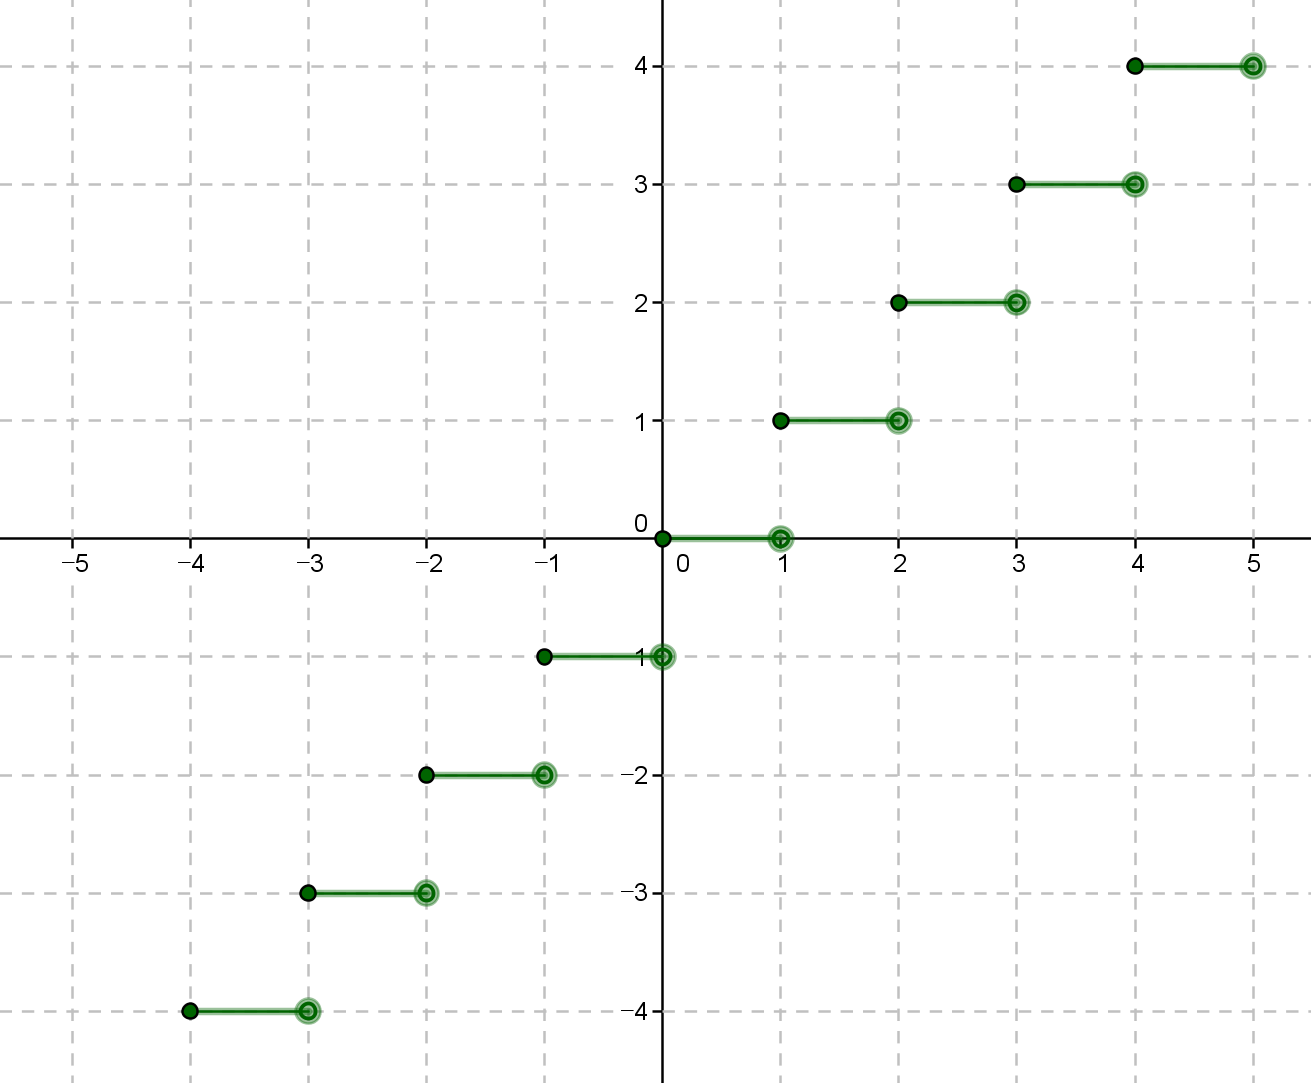
\includegraphics[width=0.7\textwidth]{13_gauss_sign}
\caption{정의 13.\ref{13_gauss_sign} \(y=[x]\)의 그래프}
\end{figure}

\theo{}
가우스기호에 대해 다음이 성립한다.
\begin{enumerate}[(1)]
\item
\(x\le y\)이면 \([x]\le [y]\)이다.
\item
\(x\le y\)라고 해서 반드시 \([x]<[y]\)는 아니다.
\item
일반적으로 \([-x]=-[x]\)이 성립하지 않는다.
\end{enumerate}

\begin{proof}
(1) 정의에 의해 \([x]\le x <[x]+1\)이고 \([y]\le y <[y]+1\)이다.
특히, \([x]\le x\le y<[y]+1\)이다.
즉 \([x]<[y]+1\)이다.
그런데 \([x]\)와 \([y]+1\)이 모두 정수이므로 두 정수의 차는 1보다 크거나 같다 ; 
\(([y]+1)-[x]\ge1\).
따라서 \([x]\le [y]\)이다.

(2) 반례 : \(x=0.2\), \(y=0.3\)이면 (2)의 가정이 성립하지만, 결론이 성립하지 않는다.

(3) 반례 : \(x=0.5\)이면 \([-x]=-1\neq0=-0=-[x]\)이다.
\end{proof}

\theo{(저울문제에 관하여, cf. p141)}
세 양수 \(a\), \(b\), \(c\)를 최대한 한 번씩만 사용하여 덧셈 혹은 뺄셈을 했을 때 만들 수 있는 양수의 개수는 최대 13개이다.
\begin{proof}
세 실수를 최대한 한 번씩만 이용하여 만들 수 있는 숫자들의 집합은
\[\{ax+by+cz|x,y,z\text{는 각각 }-1,0,1\text{ 중에 하나}\}\]
이다.
즉 다음과 같은 숫자들이다;
\[\begin{tabular}{ccc}
-a-b-c		&-b-c		&a-b-c\\
-a-b			&-b			&a-b\\
-a-b+c		&-b+c		&a-b+c\\
-a-c			&-c 			&a-c\\
-a			&0			&a\\
-a+c			&c 			&a+c\\
-a+b-c		&b-c			&a+b-c\\
-a+b			&b			&a+b\\
-a+b+c		&b+c			&a+b+c\\
\end{tabular}\]
위의 수들을 잘 살펴보면, 27개 수 중 0을 제외한 26개의 수들은 각각 \(x\)와 \(-x\)꼴의 짝을 이루고 있다.
즉 두 개의 수들 중 하나는 양수이고 하나는 음수이다.
따라서 양수 전체의 개수는 13개이다.
\end{proof}

%%
\newpage
\section{실수}
%
\defi{유리수}
정의 2. \ref{02_natural_and_integer}에서 \(\mathbb N=\{1,2,3,\cdots\}\), \(\mathbb Z=\{\cdots,-3,-2,-1,0,1,2,3,\cdots\}\)를 각각 자연수(自然數, natural number)의 집합, 정수(整數, integer)의 집합이라고 정의했다.
이제 집합
\[\mathbb Q=\left\{\frac pq\;\big|\;p,q\in Z,q\neq0\right\}\]
을 유리수의 집합이라고 정의하고 \emph{유리수(有理數, rational number)}를 \(\mathbb Q\)의 원소라고 정의하자.
즉
\[x\text{는 유리수이다.}\iff x\in\mathbb Q\]
이다.

%
\defi{유한소수와 무한소수, 순환소수와 비순환소수}
임의의 실수 \(x\)가 십진법으로 다음과 같이 표현되었다고 하자.
\[x=a_na_{n-1}\cdots a_0.b_1b_2b_3\cdots.\]
즉 \(a_i\)는 \(10^i\)자릿수를, \(b_j\)는 소수점 \(j\)번째 자리수를 나타낸다.
어떤 자연수 \(N\)에 대해 \(j\ge N\)이면 \(b_j=0\)일 때, \(x\)를 \emph{유한소수}라고 부른다.
그렇지 않은 경우, 즉 그러한 자연수 \(N\)이 존재하지 않을 때 \(x\)를 \emph{무한소수}라고 부른다.

\(x\)가 무한소수라고 가정하자.
\(b_i\)들이 일정한 규칙으로 반복될 때 \(x\)를 \emph{순환소수}라고 한다.
즉 어떤 자연수 \(k\)와 \(m\)가 존재해서 모든 자연수 \(i\)와  \(0\le j<k\)를 만족하는 \(j\)에 대해 \(b_{m+(ik+j)}=b_{m+j}\)일 때 \(x\)를 순환소수라고 부른다.
예를 들어 \(3.214141414\cdots\)는 순환소수이다.
모든 자연수 \(i\)와 \(j(=0,1)\)에 대해 \(b_{1+(2i+j)}=b_{1+j}\)이기 때문이다.

\(x\)가 무한소수이면서 순환소수가 아니면 \emph{비순환소수}라고 부른다.

%
\theo{유한소수와 순환소수는 유리수이다.}
\begin{proof}
유한소수가 유리수인 것은 당연하다.
\(x\)가 순환소수라고 가정하자.
그러면
\[\begin{array}{r@{=}r@{.}l}
x 		&a_na_{n-1}\cdots a_0					&b_1b_2\cdots b_kb_{k+1}\cdots\\
10^{k-1}x 	&a_na_{n-1}\cdots a_0b_1b_2\cdots b_{k-1}	&b_kb_{k+1}\cdots\\
10^{2k-1}x	&a_na_{n-1}\cdots a_0b_1b_2\cdots b_{2k-1}	&b_{2k}b_{2k+1}\cdots
\end{array}\]
따라서 \(10^{2k-1}x-10^{k-1}x\)은 정수이다.
즉
\[[10^{2k-1}-10^{k-1}]x=N\]
이고(\(N\)은 정수), 따라서
\[x=\frac N{10^{2k-1}-10^{k-1}}\]
는 유리수이다.
\end{proof}
여기서 증명하지는 않겠지만, 모든 유리수는 유한소수이거나 순환소수이다.
따라서 유리수의 집합 \(\mathbb Q\)는 유한소수의 집합과 순환소수의 집합의 합집합과 정확히 일치한다.

%
\defi{무리수와 실수}
\(x\)가 비순환소수이면 \(x\)를 \emph{무리수(無理數, irrational number)}라고 부른다.
무리수와 유리수를 합쳐서 \emph{실수(實數, real number)}라고 부른다.

%
\theo{유리수와 무리수의 조밀성}
유리수와 무리수는 실수 내에서 조밀하다.
즉, 임의의 서로 다른 두 실수 \(a\)와 \(b\)에 대해(\(a<b\))
\(a<x<b\)를 만족하는 유리수 \(x\)가 존재하고,
\(a<y<b\)를 만족하는 무리수 \(y\)도 존재한다.

\begin{proof}
증명은 생략한다.
p153--154의 예제 3, 4에 이 정리보다는 약한 정리가 증명되어 있다.
\end{proof}

사실 `실수가 무엇이냐'하는 문제는 생각보다 상당히 복잡하고 어려운 문제이다.
위에서는 `모든 숫자는 10진법으로 표현될 수 있다'는 가정 하에 유리수와 무리수를 분류했을 뿐이다.
하지만 그 `숫자'라는 게 무엇이냐고 물으면 답하기가 쉽지 않다.

실제로 실수 집합 \(\mathbb R\)이란 덧셈과 곱셈의 두 가지 이항연산과 부등호라는 이항관계를 가지고 있는 집합으로서, 몇 가지 공리를 만족시키는 집합으로 정의된다.

그 중 몇 가지 공리는 이미 언급했다.
덧셈과 곱셈에 관해서는 공리 6. \ref{06_number_axiom}에서 언급했다.
차례로 `덧셈의 교환법칙', `덧셈의 결합법칙', `곱셈의 교환법칙', `곱셈의 결합법칙', `덧셈과 곱셈의 분배법칙'이라고 부른다.

부등호에 대해서는 공리 4. \ref{04_inequality_axiom_1}, 4. \ref{04_inequality_axiom_2}에 대해서 언급한 바 있다.

%
\theo{}
\(a\), \(b\), \(c\), \(d\)가 유리수이고 \(\alpha\)가 무리수일 때
\begin{enumerate}[(1)]
\item
\(a+b\alpha=0\iff a=0\;\&\;\;b=0\)
\item
\(a+b\alpha=c+d\alpha\iff a=c\;\;\&\;\;b=d\)
\end{enumerate}

\begin{proof}
각각 p153--154의 예제 5, 6이다.
(2)는 (1)로부터 바로 도출할 수 있다.
\end{proof}

%
\theo{}
\(a\), \(b\), \(c\), \(d\)가 유리수이고 \(\sqrt b\), \(\sqrt d\)가 무리수일 때
\[a+\sqrt b=c+\sqrt d\iff a=c\;\;\&\;\;b=d\]
이다.

\begin{proof}
154의 예제 7이다.
\end{proof}

%%
\newpage
\section{거듭제곱근식과 지수}
%
\defi{자연수 지수\label{15_natural_exponent}}
실수 \(a\)와 자연수 \(n\)에 대해 \(a^n\)을
\begin{align*}
a^1&=a\\
a^2&=a\times a\\
a^3&=a\times a\times a\\
\vdots
\end{align*}
등으로 정의한다.

%
\defi{정수 지수\label{15_integer_exponent}}
실수 \(a\)와 정수 \(n\)에 대해 \(a^n\)을 다음과 같이 정의한다.
만약 \(n>0\)이면 정의 15.\ref{15_natural_exponent}에서처럼 정의한다.
만약 \(n=0\)이면 \(a^n=a^0=1\)로 정의한다.
만약 \(n<0\)이면 \(a^n=\frac1{a^{-n}}\)로 정의한다.
세 번째 경우 \(-n>0\)이므로 \(a^{-n}\)가 정의되는 데는 문제가 없다는 점에 주목하자.

%
\theo{지수법칙(정수)\label{15_law_of_exponents_1}}
실수 \(a\), \(b\), 정수 \(m\),  \(n\)에 대해
\begin{enumerate}[(1)]
\item
\(a^mb^n=a^{m+n}\)
\item
\((a^m)^n=a^{mn}\)
\item
\((ab)^m=a^mb^m\)
\item
\((\frac ab)^m=\frac{a^m}{b^m}\)(\(b\neq0\))
\end{enumerate}

\begin{proof}
증명은 생략한다.
\(m\), \(n\)이 각각 자연수일 때 네 법칙을 먼저 증명한 후 이를 토대로 정수 지수에 대해서 다시 증명하면 된다.
\end{proof}

%
\defi{거듭제곱근\label{15_n-th_root}}
\(a\)가 실수이고 \(n\)이 자연수일 때
\(x^n=a\)를 만족시키는 실수 \(x\)를 \emph{\(a\)의 \(n\)제곱근}이라고 부른다.

%
\theo{거듭제곱근의 존재\label{15_existence_of_n-th_root}}
정의 15. \ref{15_n-th_root}에서
\begin{enumerate}[(1)]
\item
\(a>0\)이면 \(x\)는 유일하게 하나 존재한다.
\item
\(a<0\)이고 \(n\)이 짝수이면 \(x\)는 존재하지 않는다.
\item
\(a<0\)이고 \(n\)이 홀수이면 \(x\)는 유일하게 하나 존재한다.
\end{enumerate}

\begin{proof}
(2)는 당연하다.
실수의 짝수승은 음수가 될 수 없기 때문이다.
(1)과 (3)의 증명은 생략한다.
\end{proof}

%
\defi{}
정리 15. \ref{15_existence_of_n-th_root}의 (1)번의 경우, \(a\)의 \(n\)제곱근을 \(\sqrt[n]a\)라고 표기한다.

%
\defi{유리수 지수\label{15_rational_exponent}}
양의 실수 \(x\)와 유리수 \(t=\frac mn\)에 대해(\(m\), \(n\)는 정수, \(n\neq0\)) \(x^t\)를 다음과 같이 정의한다.
만약 \(m=1\)이면 \(x^t=x^{\frac1n}=\sqrt[n]a\)로 정의한다.
일반적으로 \(m\)이 정수이면 \(x^t=x^{\frac mn}=(x^{\frac1n})^m\)으로 정의한다.

\(x\)가 음수이면 지수를 정의하기가 어려우므로 생각하지 않는다.

%
\theo{지수법칙(유리수)\label{15_law_of_exponents_2}}
양의 실수 \(a\), \(b\), 유리수 \(s\),  \(t\)에 대해
\begin{enumerate}[(1)]
\item
\(a^sb^t=a^{s+t}\)
\item
\((a^s)^t=a^{st}\)
\item
\((ab)^s=a^sb^s\)
\item
\((\frac ab)^s=\frac{a^s}{b^s}\)(\(b\neq0\))
\end{enumerate}
\begin{proof}
정리 15. \ref{15_law_of_exponents_1}를 사용하여 약간의 계산을 거치면 어렵지 않게 증명할 수 있다.
\end{proof}

%
\theo{실수 지수}
고등학교 과정의 극한 개념을 이용하면 실수 지수도 정의할 수 있다.
예를 들어, \(3^{\sqrt2}\)를 정의해보자.
\(\sqrt2=1.414213\cdots\)이다.
따라서 다음과 같은 수의 열을 생각해보자.
\begin{align*}
x_1&=3^1=3\\
x_2&=3^{1.4}=4.65553672175\cdots\\
x_3&=3^{1.41}=4.70696500172\cdots\\
x_4&=3^{1.414}=4.72769503527\cdots\\
x_5&=3^{1.4142}=4.72873393017\cdots\\
x_6&=3^{1.41421}=4.72878588091\cdots\\
x_7&=3^{1.414213}=4.72880146624\cdots\\
\vdots
\end{align*}
위 식들의 우변은 정의 15. \ref{15_rational_exponent}에 의하여 잘 정의되어 있다는 점에 주목하자.
이 수열(=수의 열)인 \(\{x_n\}\)은 \(n\)이 증가할수록 일정한 값에 가까워지는 것처럼 보인다.
이 값을 이 수열의 `극한'이라고 부른다.
그리고 이 극한값을 \(3^{\sqrt2}\)로 정의한다.


%
\theo{지수법칙(실수)}
양의 실수 \(a\), \(b\), 실수 \(s\),  \(t\)에 대해
\begin{enumerate}[(1)]
\item
\(a^sb^t=a^{s+t}\)
\item
\((a^s)^t=a^{st}\)
\item
\((ab)^s=a^sb^s\)
\item
\((\frac ab)^s=\frac{a^s}{b^s}\)(\(b\neq0\))
\end{enumerate}
\begin{proof}
정리 15. \ref{15_law_of_exponents_2}와 극한의 성질을 사용하여 증명할 수 있다.
\end{proof}
\end{document}